\chapter{Parser}

In this chapter the requirements for NISSE will be presented, along with the CFG hereof.

\section{Requirements}
The requirements for the NISSE parser are:
\begin{itemize}
	\item The parser should be able to receive tokens from the lexer, which it then can convert into a parse tree.
	\item It should be able to report useful error messages if the user has written something illegal according to the CFG of NISSE.
	\item The CFG should be unambiguous, such that it is possible to make a parser for it. 
\end{itemize}

\newpage
\section{CFG}
\begin{lstlisting}[frame=single, caption={CFG of NISSE in EBNF.}, label={lst:ebnf}, language=NISSE]
SS              = Blocks ;
Blocks          = BeginBlock {Lines} Endblock | SettingBlock ;
Lines           = SettingBlock | Numeration | Itemlist | Plains eol ;
Numeration      = nlist (Plains eol | Numeration) ;
Itemlist        = blist (Plains eol | Itemlist) ;
BeginBlock      = beginkwd {space} BEBlock eol ;
EndBlock        = endkwd {space} BEBlock eol ;
BEBlock         = lcurly {space} char {space} [BEBlockv1] rcurly ;
BEBlockv1       = pipe {space} char {space}  ;
SettingBlock    = settingkwd lcurly ShortIdent {space} pipe {space} char {space} rcurly {space} eol ;
Plains          = (ShortBlock | CharAll) {(ShortBlock | CharAll)} ;
ShortBlock      = format_kwd lcurly {space} [ShortIdents] Plains rcurly ;
ShortIdents     = ShortIdent pipe ;
ShortIdent      = Kwd {space} colon {space} ShortIdentv1,{ShortIdentv1} {space} ;
ShortIdentv1    = char | digit | Float | colon | fslash | dot ;
Kwd             = atsign char | url ;
CharAll         = colon | digit | scolon | percent | fslash | bslash | exclamation | dot | comma | char | space | underscore | hyphen;
Float           = digit dot digit ; 
eol             = eolv1 , {eolv1} ;
dot             = dotv1 , {dotv1};
comma           = commav1,{commav1} ;
\end{lstlisting}
Listing \ref{lst:ebnf} shows the CFG for NISSE in EBNF. With the rules of table \ref{tbl:EBNFSyntax}.

NISSE's grammar is able to construct everything that is required of NISSE. \\
\begin{figure}[! h]
\centering
	 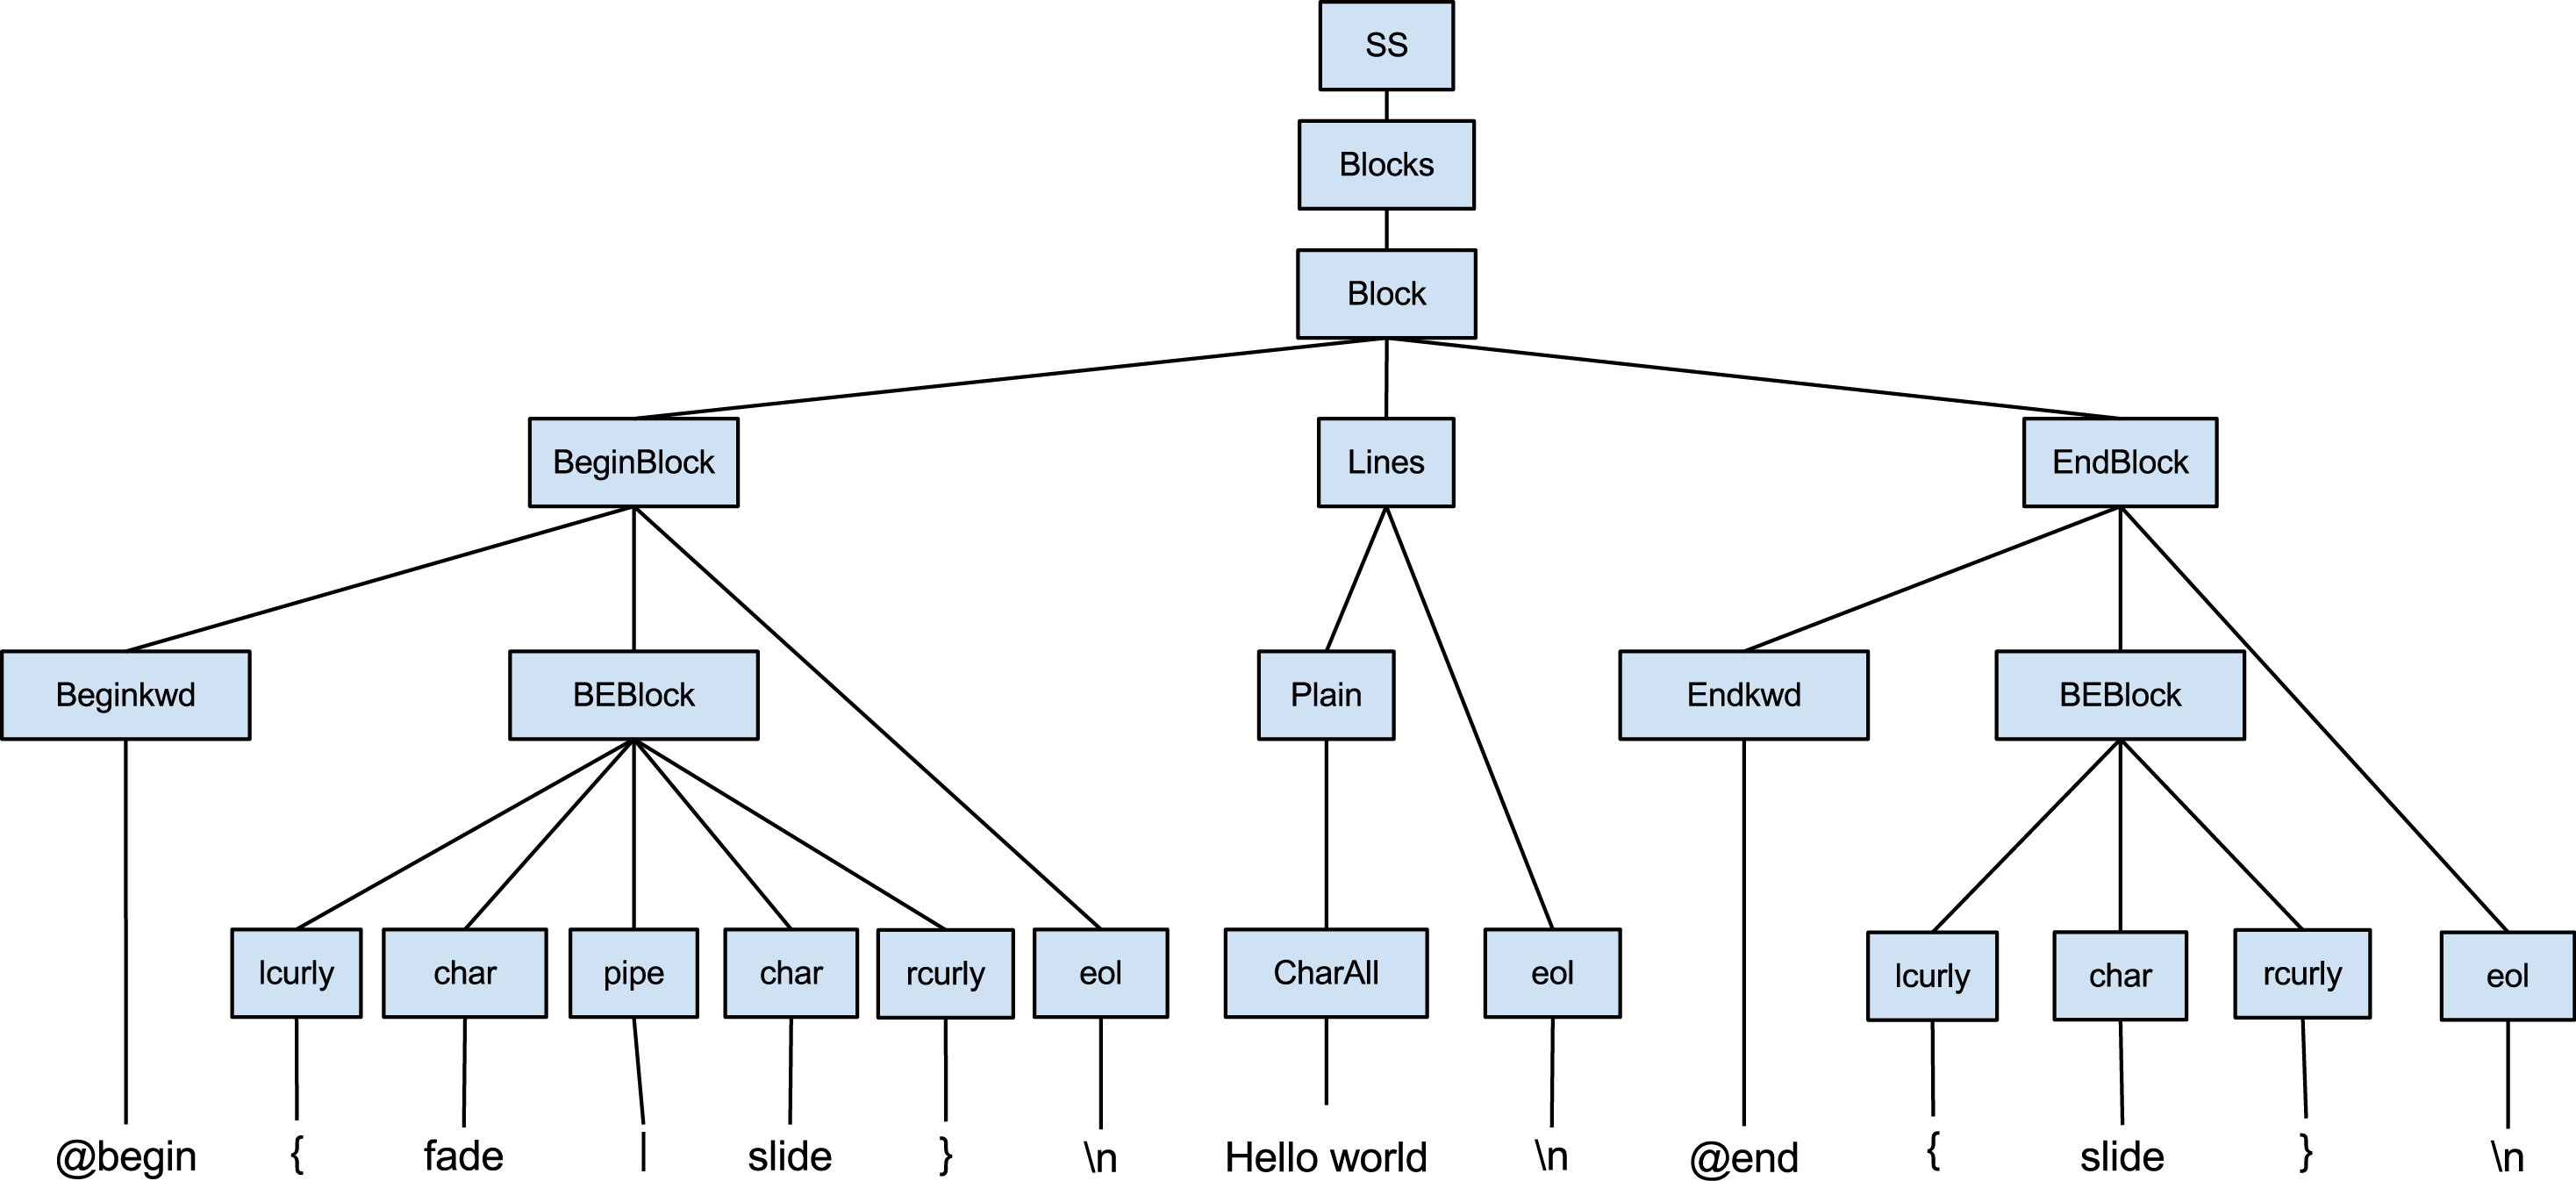
\includegraphics[width=350px]{images/ebnfexample.png}
		 \caption{Parse tree for a simple slide.}	
	\label{fig:Parsetree}
\end{figure}
Figure \ref{fig:Parsetree} shows how the CFG would parse the AST, with the input of listing \ref{lst:BasicElemets}.
\section{Conclusion}
The CFG is concluded to be LALR according to section \ref{Parserstrategy}, the CFG is not ambiguous either, as per the definition of LALR (\cite{CaC} Chapter 6).

\noindent{The grammar for the language is LL(1) according to the tool called ``kfG Edit'', which was introduced in a lecture. Later it was tested if the grammar was LALR(1) by using SableCC to try and generate a parser, and it was proved that the grammar was LALR(1). ``kfG Edit’’ uses a special syntax that can be seen in appendix \ref{AkfG}.